\section{EXAMINATION OF THE UNCONSOLIDATED-UNDRAINED TEST 不固结不排水试验\protect\footnote[6]{
    The following two sections on UU and CU Tests are restricted to normally consolidated clays of moderate sensitivity, although the concepts can be extended to overconsolidated clays. 以下有关UU和CU试验的两节仅限于中等敏感度的正常固结黏土,尽管这些概念可以扩展到超固结黏土。
}}

\begin{paracol}{2}
    
    The test data in \autoref{figure:5} through \autoref{figure:8} indicate that soil tested in unconsolidatedundrained shear resembles, in several respects, the results of tests on overconsolidated clays. In particular, the $\overline{UU}$ data show: 

    \switchcolumn

    图中的试验数据。 \cnfigureref{figure:5}至\cnfigureref{figure:8}表明,在非固结不排水的剪切中试验的土壤在某些方面类似于对超固结黏土的试验结果。 特别是,$\overline{UU}$数据显示:

    \switchcolumn*

    \begin{enumerate}
        \item Values of undrained shear strength for a given initial effective stress $\overline{\sigma}_r$ which are above the corresponding values for normally consolidated clay; 
        \item Effective stress paths during shear which move upward and to the right since the pore pressure parameter $A$ is less than one half, a characteristic of overconsolidated clay;
    \end{enumerate}

    \switchcolumn
    
    \begin{enumerate}
        \item 对于给定的初始有效应力$\overline{\sigma}_r$,不排水的剪切强度值高于正常固结黏土的相应值; 
        \item 由于孔隙压力参数$A$小于1/2,因此在剪切过程中有效应力路径向上和向右移动,这是黏土的超固结特征。 
    \end{enumerate}

    \switchcolumn*
    
    The similarity between the results of $\overline{UU}$ tests and tests on overconsolidated specimens is presented in \autoref{figure:11} for Kawasaki clays. In \autoref{figure:11b} $CA-\overline{UU}$ tests represent the undrained strength of perfect specimens, preshear $\overline{\sigma}=\overline{\sigma}_{ps}$, whereas the UU tests show the strength of actual specimens, preshear $\overline{\sigma}=\overline{\sigma}_r$. This figure shows that the effective stress paths for the $\overline{UU}$ tests, \autoref{figure:11b}, when normalized by dividing by $\overline{\sigma}_{ps}$, are similar in shape to the effective stress paths of 的$\overline{CIU}$ tests on overconsolidated clays shown in \autoref{figure:11a}, when normalized by dividing by $\overline{\sigma}_{cm}$. In other words, the reduction in effective stress from $\overline{\sigma}_{ps}$ to $\overline{\sigma}_r$ caused by sample disturbance and the reduction in effective stress from $\overline{\sigma}_{cm}$ to $\overline{\sigma}_c$ caused by rebound appear to have comparable effects on undrained strength.

    \switchcolumn
    
    对于Kawasaki黏土,$\overline{UU}$试验结果与超固结试样试验之间的相似性在\cnfigureref{figure:11}中给出。 在\cnsubfigureref{figure:11b}中,$CA-\overline{UU}$试验代表理想试样的不排水强度,预剪切力$\overline{\sigma}=\overline{\sigma}_{ps}$,而$\overline{UU}$试验则表明实际试样的强度,预剪切力$\overline{\sigma}=\overline{\sigma}_r$。 该图表明,通过除以$\overline{\sigma}_{ps}$进行归一化后,$\overline{UU}$试验的有效应力路径\cnsubfigureref{figure:11b}的形状类似于\cnsubfigureref{figure:11a}中对超固结黏土的$\overline{CIU}$试验的有效应力路径,然后除以$\overline{\sigma}_{cm}$。换句话说,由样品扰动引起的有效应力从$\overline{\sigma}_{ps}$到$\overline{\sigma}_r$的减小和由回弹引起的有效应力从$\overline{\sigma}_{cm}$到$\overline{\sigma}_c$的减小似乎对不排水强度具有类似的影响。

\end{paracol}

\begin{figure}[!htbp]
    \centering
    \subfigure[EFFECT OF O.C.R. OCR的作用]{
        \label{figure:11a}
        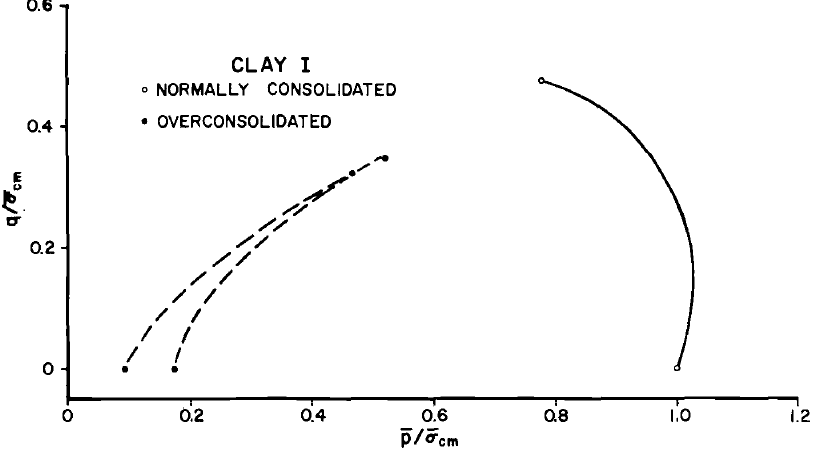
\includegraphics[width=0.48\textwidth]{figures/figure-11a.png}
    }
    \subfigure[EFFECT OF SAMPLING 采样的作用]{
        \label{figure:11b}
        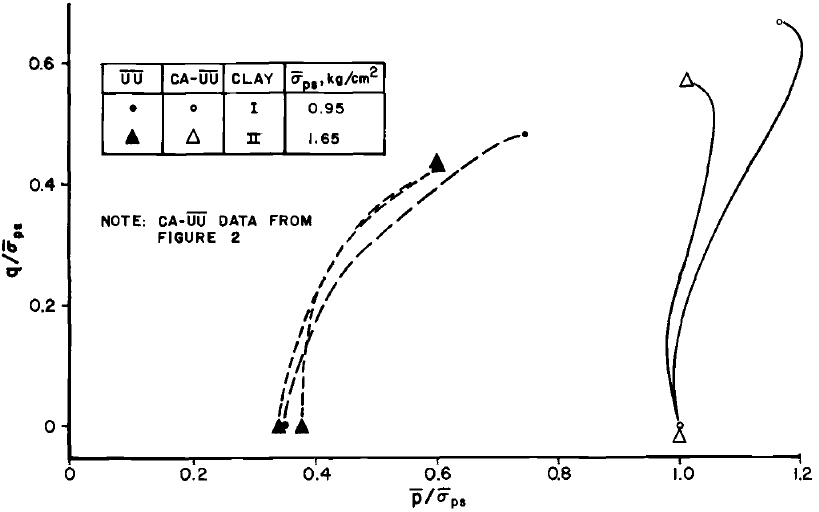
\includegraphics[width=0.48\textwidth]{figures/figure-11b.png}
    }
    \caption{Stress Paths for Kawasaki Clays.}
    \addtocounter{figure}{-1}
    \vspace{-5pt}
    \renewcommand{\figurename}{图}
    \caption{Kawasaki黏土的应力路径。}
    \renewcommand{\figurename}{Figure}
    \label{figure:11}
\end{figure}

\begin{paracol}{2}
    
    This analogy suggests that the strength from UU tests can be considered as test results on overconsolidated specimens with a maximum past pressure equal to $\overline{\sigma}_{ps}$, the value of effective stress existing before gross sample disturbance occurred (see Point P in \autoref{figure:3}). Thus the corrected value of $S_u$ from UU tests, which will correspond to the strength of a specimen after perfect sampling, can be estimated by treating the ratio of $\overline{\sigma}_{ps}$ to $\overline{\sigma}_r$, as an overconsolidation ratio.

    \switchcolumn

    这种类比表明,UU试验的强度可以看作是对超固结试样的试验结果,该试样的最大过去压力等于$\overline{\sigma}_{ps}$,即发生总样本扰动之前存在的有效应力值(参见\cnfigureref{figure:3}中的P点)。 因此,通过将$\overline{\sigma}_{ps}$与$\overline{\sigma}_r$的比值视为过固结率,可以估算出UU试验的$S_u$的校正值,该值对应于完美采样后样品的强度。

    \switchcolumn*

    The proposed method of correcting the undrained shear strength for sample disturbance involves the following three steps: 

    \switchcolumn
   
    校正样品扰动的不排水剪切强度的建议方法包括以下三个步骤:

    \switchcolumn*

    \begin{enumerate}
        \item Relate undrained shear strength to overconsolidation ratio using CIU tests on specimens with $\overline{\sigma}_{cm}$ much greater than $\overline{\sigma}_{v0}$ to reduce the effects of disturbalice, 
        \item Find the equivalent overconsolidation ratio for the UU test being corrected by measuring $\overline{\sigma}_r$ and calculating $\overline{\sigma}_{ps}$, (use \autoref{equation:1} and $CA-\overline{UU}$ data or estimates from \autoref{table:1}), and
        \item Obtain the shear strength correction for the particular overconsolidation ratio as described below.
    \end{enumerate}

    \switchcolumn
    
    \begin{enumerate}
        \item 使用CIU试验对$\overline{\sigma}_{cm}$远大于$\overline{\sigma}_{v0}$的样品考虑不排水剪切强度与超固结率的相关性,以减少干扰的影响,
        \item 通过测量$\overline{\sigma}_r$并计算$\overline{\sigma}_{ps}$,找到要校正的UU试验的等效超固结比(使用\cnequationref{equation:1}和$CA-\overline{UU}$数据或\cntableref{table:1}的估计值),
        \item 获得特定超固结比的抗剪强度修正值,如下面所描述的。
    \end{enumerate}

    \switchcolumn*

    \autoref{figure:12} presents the ratio of undrained shear strength at $\overline{\sigma}_c$ to the strength at $\overline{\sigma}_{cm}$ versus overconsolidation ratio for CIU tests on several natural and remolded clays. As can be seen, the strength ratio decreases significantly with an increase in OCR. Considering the ratio of $\overline{\sigma}_{ps}$ to $\overline{\sigma}_r$ equivalent to OCR, one can read from such a figure the loss in shear strength from excessive sample disturbance which reduces the effective stress from $\overline{\sigma}_{ps}$ to $\overline{\sigma}_r$. From the residual effective stress data already discussed, a typical value of $\overline{\sigma}_r/\overline{\sigma}_{ps}$ might be $\frac{1}{3}$ to $\frac{1}{4}$, the equivalent OCR would then be 3 to 4. Using the data in \autoref{figure:12}, one sees that measured values of UU strength would therefore be 20 to 50 percent too low depending on the type of clay.

    \switchcolumn

    \cnfigureref{figure:12}显示了在几种天然和重塑黏土上进行CIU试验时,$\overline{\sigma}_c$时不排水的剪切强度与$\overline{\sigma}_{cm}$时的强度之比与超固结比。 可以看出,强度比随着OCR的增加而显着降低。 考虑到$\overline{\sigma}_{ps}$与$\overline{\sigma}_r$的比值等于OCR,可以从该图中读取由于过度的样品扰动而导致的剪切强度损失,从而将有效应力从$\overline{\sigma}_{ps}$减小到$\overline{\sigma}_r$。从已经讨论过的残余有效应力数据来看,典型的$\overline{\sigma}_r/\overline{\sigma}_{ps}$值可能是$\frac{1}{3}$到$\frac{1}{4}$,那么等效的OCR就是3到4。使用\cnfigureref{figure:12}中的数据,可以看到,根据黏土的类型,UU强度可能会因此下降20$\%$至50$\%$。

\end{paracol}

\begin{figure}[!htb]
    \centering
    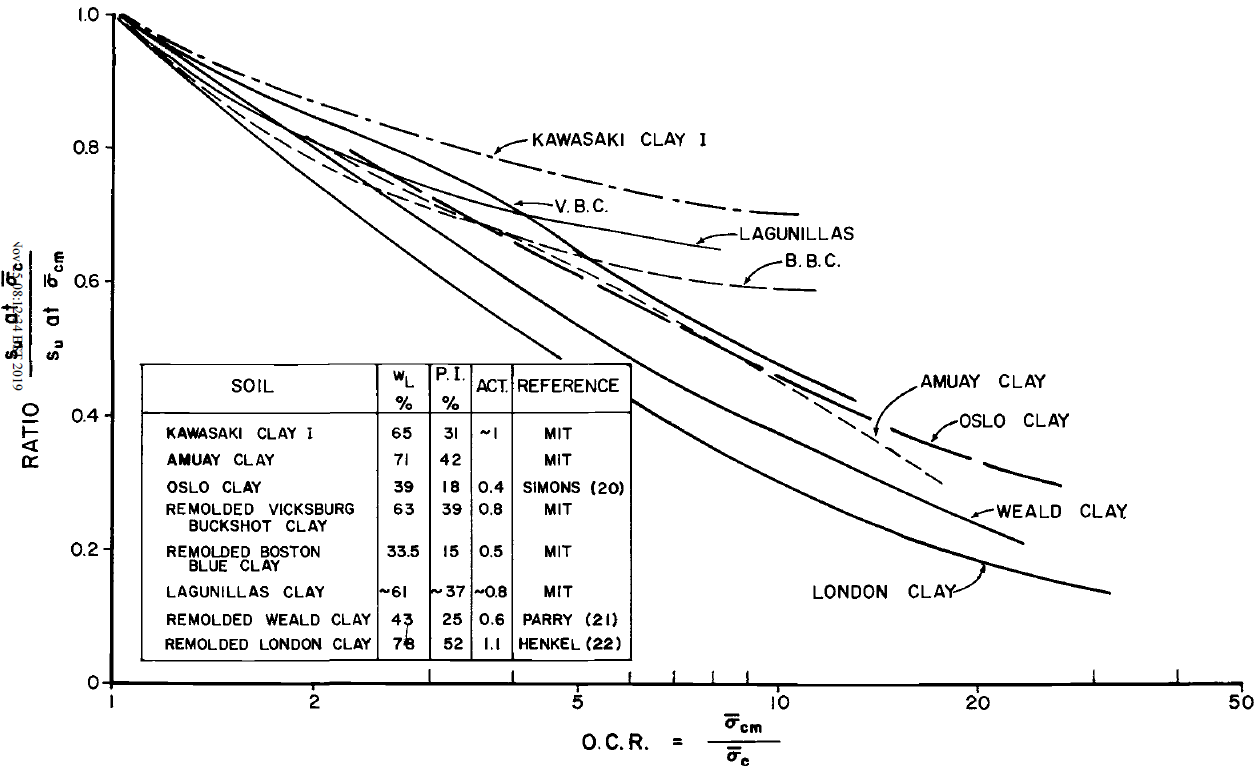
\includegraphics[width=0.7\textwidth]{figures/figure-12.png}
    \caption{Effect of OCR on Undrained Strength.}
    \addtocounter{figure}{-1}
    \vspace{-5pt}
    \renewcommand{\figurename}{图}
    \caption{OCR对不排水强度的影响。}
    \renewcommand{\figurename}{Figure}
    \label{figure:12}
\end{figure}

\begin{paracol}{2}

    Considering a UU test as a test on an overconsolidated specimen is thought to be an important concept. To correct the results of UU tests by use of an equivalent overconsolidation ratio is proposed as an approximate engineering approach. There are both theoretical and practical reasons why such an approach is not precise. Of greatest consequence, it is probably unwarranted to assume with the present state of knowledge that all of the detrimental effects of sampling can be expressed simply as a reduction in effective stress. Further, accurate methods for determining $\overline{\sigma}_{ps}$ are not currently known. Had the specimen existed at a possibly varying $K_0$ effective stress system for a geological time rather than for the time used in the laboratory for a $CA-\overline{UU}$ test, the value of effective stress following perfect sampling might be different. There is also the added problem of the variability in $\overline{\sigma}_r$ measurements. However, to the authors' knowledge, no other method exists for the quantitative evaluation of the very significant effects of disturbance on UU strengths.

    \switchcolumn
        
    将UU试验视为对超固结试样的试验是一个重要的概念。 为了使用等效的超固结比来校正UU试验的结果,建议将其作为一种近似的工程方法。 从理论上和实践上来看,这种方法都不精确。 最重要的结果是,根据目前的知识状况,可能没有必要假设采样的所有有害影响都可以简单地表示为有效压力的降低。 此外,当前没有用于确定$\overline{\sigma}_{ps}$的精确方法。 如果样本存在一个可能变化的$K_0$有效应力系统一段地质时间,而不是在实验室中用于$CA-\overline{UU}$试验的时间,那么完美采样后的有效应力值可能会有所不同。 $\overline{\sigma}_r$测量中的可变性也存在另一个问题。 但是,据作者所知,没有其他方法可以定量评估扰动对UU强度的非常显着的影响。

\end{paracol}